\documentclass[a2paper, 12pt]{article}
\usepackage[font={huge, bf}]{caption}
\usepackage{fontspec}
\setmainfont{Arial}
\usepackage{subcaption}
\usepackage{graphicx}
\usepackage{tikz}
\usepackage{tikzsymbols}
\usetikzlibrary{calc,patterns,shapes.geometric}
\usepackage{float}
\usepackage{pdflscape}
\usepackage{geometry}
\geometry{landscape, margin=2cm}
\captionsetup[subfigure]{justification=justified,singlelinecheck=false}
\pagestyle{empty}

\def\centerarc[#1](#2)(#3:#4:#5){\draw[#1] ($(#2)+({#5*cos(#3)},{#5*sin(#3)})$) arc (#3:#4:#5);}

\begin{document}
	\vspace*{\fill}
	\begin{figure}[!htbp]
		\centering
		\begin{subfigure}[b]{0.48\textwidth}
			\caption{Figure 1}
			\centering
			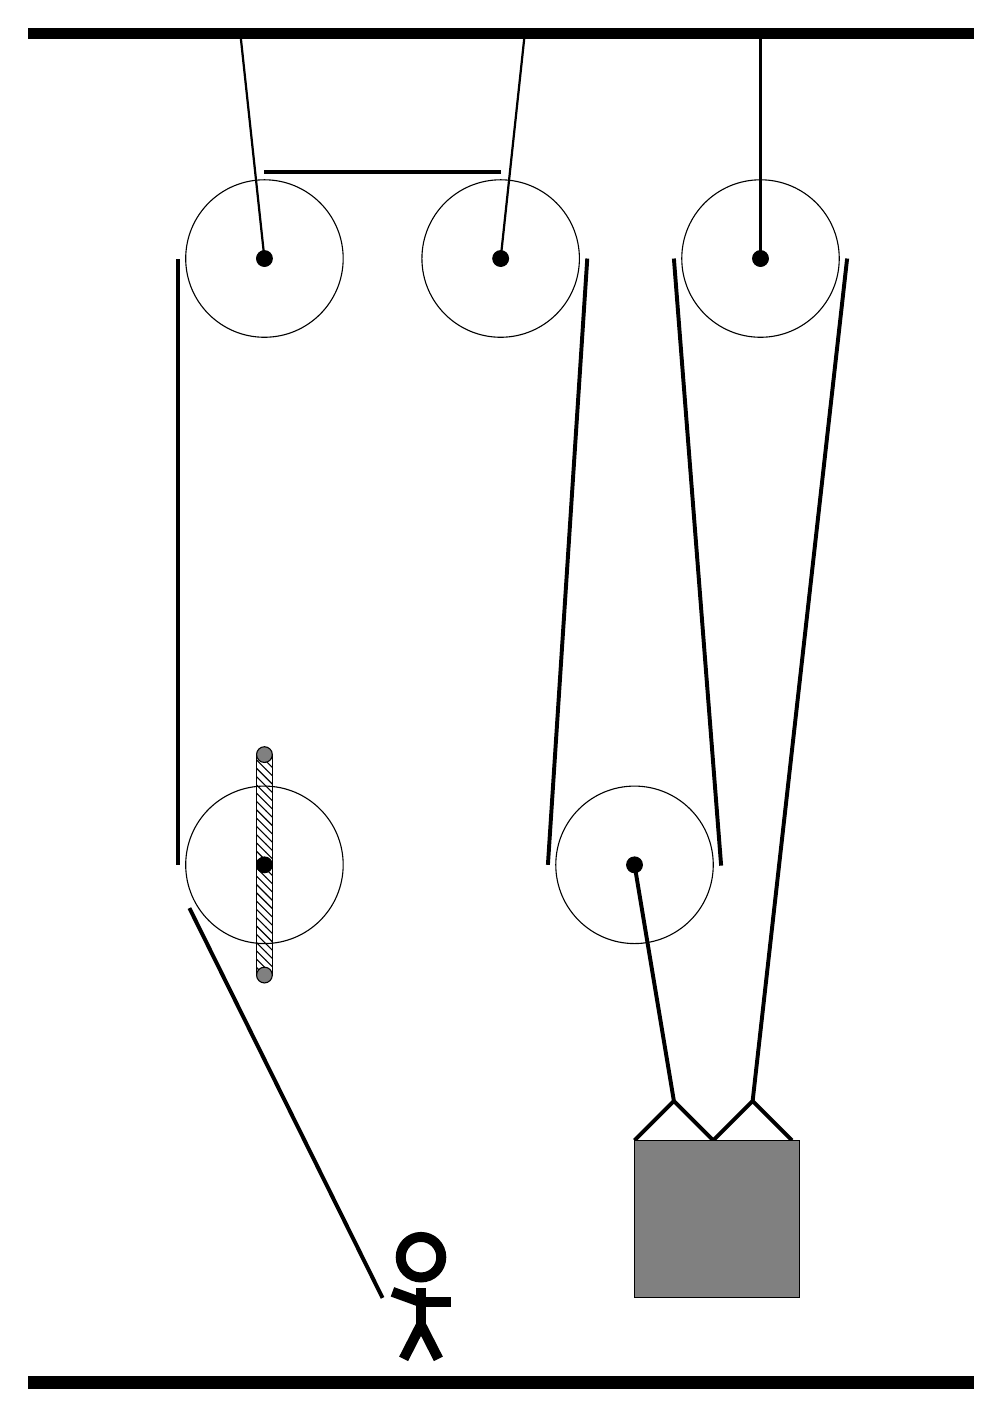
\begin{tikzpicture}
				\draw[fill=black] (-5, 14) rectangle (7, 14.125);
				
				\draw (1, 11.2) circle (1);
				\draw[fill=black] (1, 11.2) circle (0.1);
				\draw[thick] (1, 11.2) -- (1.3, 14);
				
				\draw (4.3, 11.2) circle (1);
				\draw[fill=black] (4.3, 11.2) circle (0.1);
				\draw[thick] (4.3, 11.2) -- (4.3, 14);
				
				\draw (2.7, 3.5) circle (1);
				\draw[fill=black] (2.7, 3.5) circle (0.1);
				
				\draw[line width=0.5mm]  (2.7, 0) -- (3.2, 0.5) -- (3.7, 0) -- (4.2, 0.5) -- (4.7, 0);
				\draw[fill=black!50] (2.7, 0) rectangle (4.8, -2);
				
				\draw (-2, 11.2) circle (1);
				\draw[fill=black] (-2, 11.2) circle (0.1);
				\draw[thick] (-2, 11.2) -- (-2.3, 14);
				
				\draw (-2, 3.5) circle (1);
				\draw[fill=black] (-2, 3.5) circle (0.1);
				\draw[pattern=north west lines, pattern color=black] (-2.1, 4.9) rectangle (-1.9, 2.1);
				\draw[fill=black!50] (-2, 4.9) circle (0.1);
				\draw[fill=black!50] (-2, 2.1) circle (0.1);
				
				\draw[line width=0.5mm](-0.5, -2) -- (-2.9526, 2.95);
				\centerarc[line width=0.5mm](-2, 3.5)(180:210:1.1);
				\draw[line width=0.5mm](-3.1, 3.5) -- (-3.1, 11.2);
				\centerarc[line width=0.5mm](-2, 11.2)(90:180:1.1);
				
				\draw[line width=0.5mm](-2, 12.3) -- (1, 12.3);
				\centerarc[line width=0.5mm](1, 11.2)(0:90:1.1);
				\draw[line width=0.5mm](2.1, 11.2) -- (1.6, 3.5);
				\centerarc[line width=0.5mm](2.7, 3.5)(180:370:1.1);
				\draw[line width=0.5mm] (3.8, 3.49) -- (3.2, 11.2);
				\centerarc[line width=0.5mm](4.3, 11.2)(0:180:1.1);
				\draw[line width=0.5mm](4.2, 0.5) -- (5.4, 11.2);
				\draw[line width=0.5mm] (3.2, 0.5) -- (2.7, 3.5);
				
				\node at (0, -2) {\scriptsize \Strichmaxerl[10][-20][0]};
				
				\draw[fill=black] (-5, -3) rectangle (7, -3.15);
			\end{tikzpicture}
		\end{subfigure}
		\hfill
		\begin{subfigure}[b]{0.48\textwidth}
			\caption{Figure 2}
			\centering
			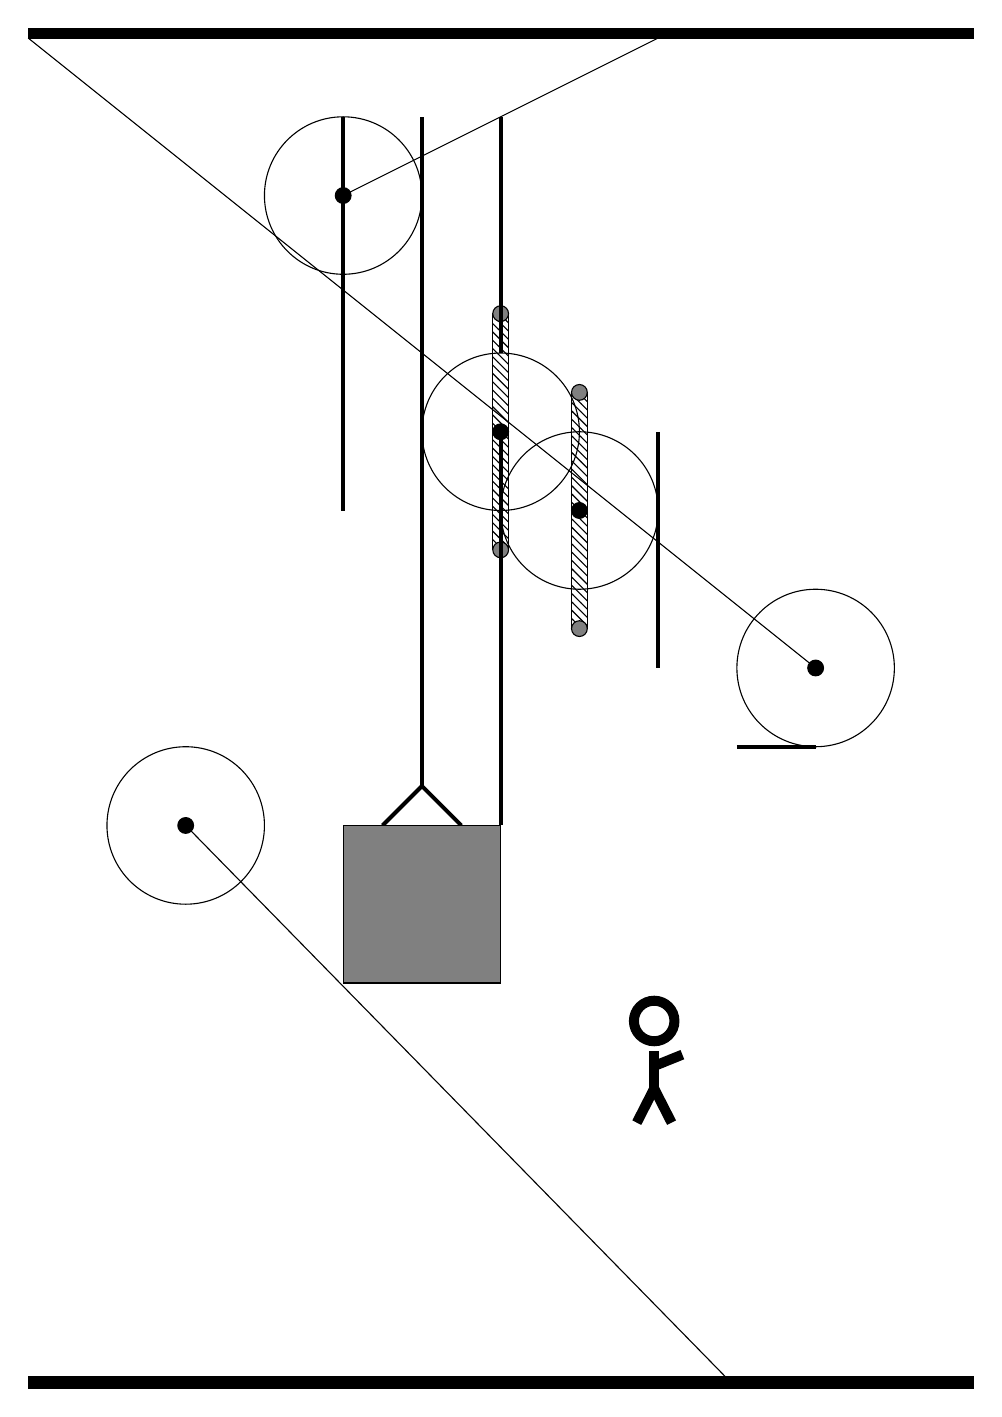
\begin{tikzpicture}
				\draw[fill=black] (-5, 14) rectangle (7, 14.125);
				
				\draw (2,8) circle (1);
				\draw[fill=black] (2,8) circle (0.1);
				\draw[pattern=north west lines, pattern color=black] (1.9,9.5) rectangle (2.1,6.5);
				\draw[fill=black!50] (2,9.5) circle (0.1);
				\draw[fill=black!50] (2,6.5) circle (0.1);
				
				\draw (1,9) circle (1);
				\draw[fill=black] (1,9) circle (0.1);
				\draw[pattern=north west lines, pattern color=black] (0.9,10.5) rectangle (1.1,7.5);
				\draw[fill=black!50] (1,10.5) circle (0.1);
				\draw[fill=black!50] (1,7.5) circle (0.1);
				
				\draw (-3,4) circle (1);
				\draw[fill=black] (-3,4) circle (0.1);
				\draw (4,-3.15) -- (-3,4);
				
				\draw (-1,12) circle (1);
				\draw[fill=black] (-1,12) circle (0.1);
				\draw (3,14.0) -- (-1,12);
				
				\draw (5,6) circle (1);
				\draw[fill=black] (5,6) circle (0.1);
				\draw (-5,14.0) -- (5,6);
				
				\draw[line width=0.5mm](0,4.5) -- (0,13.0);
				\draw[line width=0.5mm](-0.5,4) --  (0,4.5) -- (0.5,4);
				\draw[fill=black!50] (-1, 4) rectangle (1, 2);
				
				\draw[line width = 0.5mm] (1,4) -- (1,9);
				\centerarc[line width = 0.5mm](2,9)(0:180:1);
				\draw[line width = 0.5mm] (3,9) -- (3,6);
				\centerarc[line width = 0.5mm](4,6)(270:180:1);
				\draw[line width = 0.5mm] (4,5) -- (5,5);
				\draw[line width = 0.5mm] (-1,8) -- (-1,13);
				\centerarc[line width = 0.5mm](0,13)(0:180:1);
				\draw[line width = 0.5mm] (1,13) -- (1,10);
				\centerarc[line width = 0.5mm](2,10)(270:180:1);
				
				\node at (3, 1) {\scriptsize \Strichmaxerl[10][90][22]};
				
				\draw[fill=black] (-5, -3) rectangle (7, -3.15);
			\end{tikzpicture}
		\end{subfigure}
	\end{figure}
		\vspace*{\fill}
\end{document}